\documentclass[letterpaper]{article}
\usepackage{natbib,alifexi}
\usepackage[utf8]{inputenc}
\usepackage{amsmath}
\usepackage[toc,page]{appendix}
\usepackage[frenchb]{babel}
\usepackage[T1]{fontenc}
\usepackage{placeins, latexsym, amssymb}
\usepackage{comment}

\usepackage[hidelinks]{hyperref}

\title{Time stretching en temps réel pour le live coding}
\author{Abdeselam El-Haman Abdeselam$^{1}$\\
Superviseur : Bernard Fortz
\mbox{}\\\\
$^1$Université Libre de Bruxelles \\
aelhaman@ulb.ac.be}

%\setlength{\parskip}{0.5em}

\begin{document}
\maketitle

\begin{abstract}
  Overtone est une libraire en Clojure qui est utilisée pour faire du
  Live Coding (l'art de programmer en \og vif \fg{}). Une des techniques les
  plus utilisées dans le domaine de la musique synthétisée est le
  time-stretching, qui consiste à rallonger ou rétrécir une pièce musicale
  sans changer sa tonalité. Le time-stretching est intéressant dans
  le live-coding lorsqu'on peut modifier les paramétres de celui-ci
  en temps réel. Dans cet article 2 méthodes de time-stretching avec des
  approches différentes seront analysées, comparées et utilisées en temps
  réel dans Overtone.

\end{abstract}

\section{Introduction}

  Depuis le débuts de la musique éléctronique, le ``resampling'' de pièces musicales
  (c'est à dire, la manipulation de celles-ci) a un rôle important pour pouvoir manipuler
  des pièces musicales (rajouter des filtres, des envelopes, etc \ldots ) [rajouter citation ici].

  Un son est un signal qui est défini par sa durée, sa fréquence et son amplitude. La fréquence
  définit son ``pitch'' ou tonalité. La tonalité d'un son est plus grave si la fréquence est plus
  petite (donc une période plus grande).
  
  La manipulation d'un son dans le temps est utilisée très souvent lors du mixage et DJing.
  Ce genre de manipulations aident à rétrécir ou prolonger cette pièce pour, par exemple, mettre
  un son à la même vitesse que le ``tempo'' d'une chanson.

  Cette manipulation aura comme résultat aussi un effet sécondaire. La prolongation du signal
  provoquera aussi que la fréquence de ce signal soit modifié, et avec ça, un changement
  de tonalité non désiré se produira.

  \begin{figure}[h]
    \centerline{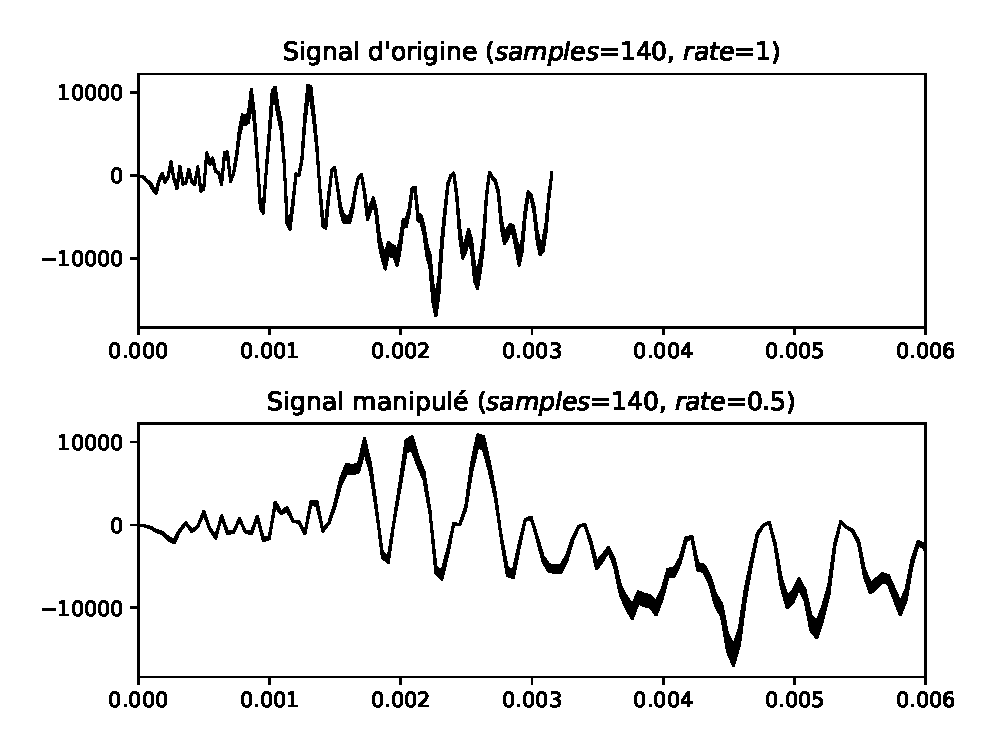
\includegraphics[width=9cm]{res/fig1.eps}}
    \caption{\label{fig:guitar-stretch}Sample d'une guitare lu à des vitesses différents}
  \end{figure}
  
  Le time-stretching est une technique pour éradiquer ce problème: changer le tempo d'un
  son sans changer sa tonalité.

  Plusieurs algorithmes existent pour implementer cette technique. Dans cet article l'état de
  l'art du time-stretching sera étudié et plusieurs de ces algorithmes seront
  implémentés pour l'application en temps réel de cette technique sur Overtone, une librairie pour
  qui a été conçue pour le traitement et synthèse de son. 

\section{État de l'art}
\subsection{Méthode OLA}
\paragraph{}En général la méthode utilisée dans les algorithmes TSM se résume en plusieures étapes
distinctes.

\paragraph{Décomposer le signal d'entrée en grains} Le signal d'entrée est décomposé en
\emph{grains} [citer article] d'une taille rélativement petite et fixe. Chacun de ces ces grains sa un décalage \emph{hopsize} $H_{a}$ (hopsize d'analyse). On peut représenter ça tel que:
$$x_m(r) = x(r + mH_{a}) : r \in [-N/2 : N/2 -1]$$
où $x$ est notre signal d'entrée en format discret de taille $L \in \mathbb{Z}_{\geq0}$. $N$ est la
taille du grain $x_m$.

La taille de ces grains doît est généralement d'une taille entre 50ms et 100ms. Ceci est important
pour trouver le \emph{pitch local} dans l'intervale $[mH_{a} - N/2 : mH_{a} + N/2 +1]$. Si l'intervale
est grand, plusieures tonalités apparaissent dans cet intervale, donc ce grain n'est pas représentatif.
\paragraph{Modifier le hopsize} Une fois le signal décomposé, avec l'information de pitch dans chaque grain, on va définir un nouveau hopsize $H_{s}$ qui va servir à récomposer ces grains. Ce $H_{s}$ est défini tel que :

$$H_{s} = \alpha H_{a}$$

Dans lequel $\alpha$ représente le \emph{facteur d'échelle}.
L'effet du TSM est fixé par le \emph{facteur d'échelle}. Pour un effet de rétrécissement:
$$\alpha < 1$$

Au contraire, pour un effet d'élargissement:
$$\alpha > 1$$

\paragraph{Superposition de grains}

Avec $H_{s}$ défini, on peut réconstruire le signal résultat de cette modification, en récomposant
le nouveau signal avec les \emph{grains} avec un décalage de $H_{s}$ au lieu de $H_{a}$. Alors ces
grains sont superposés avec une différence de $H_{s}$ et additionés. C'est à dire:

$$ y(t) = \sum_{m \in \mathbb{Z}} x_{m}(t-mH_{s})$$

où $y(t)$ est le signal de sortie par rapport au temps $t$.
u
\paragraph {Fenêtrage}

Hormis le fait que cette méthode est utilisée comme base des algorithmes qui seront illustrés plus
tard dans ce document, elle crée beaucoup d'\emph{artéfacts} à cause d'un déphasage entre les
grains qui provoque des discontinuités qui se traduit par des sons lourds et courts qui n'étaient pas
dans le signal initial. Ceci est dû à cause d'un déphasage important entre les grains
puisque $H_{s} \neq H_{a}$.

\begin{figure}[h]
    \centerline{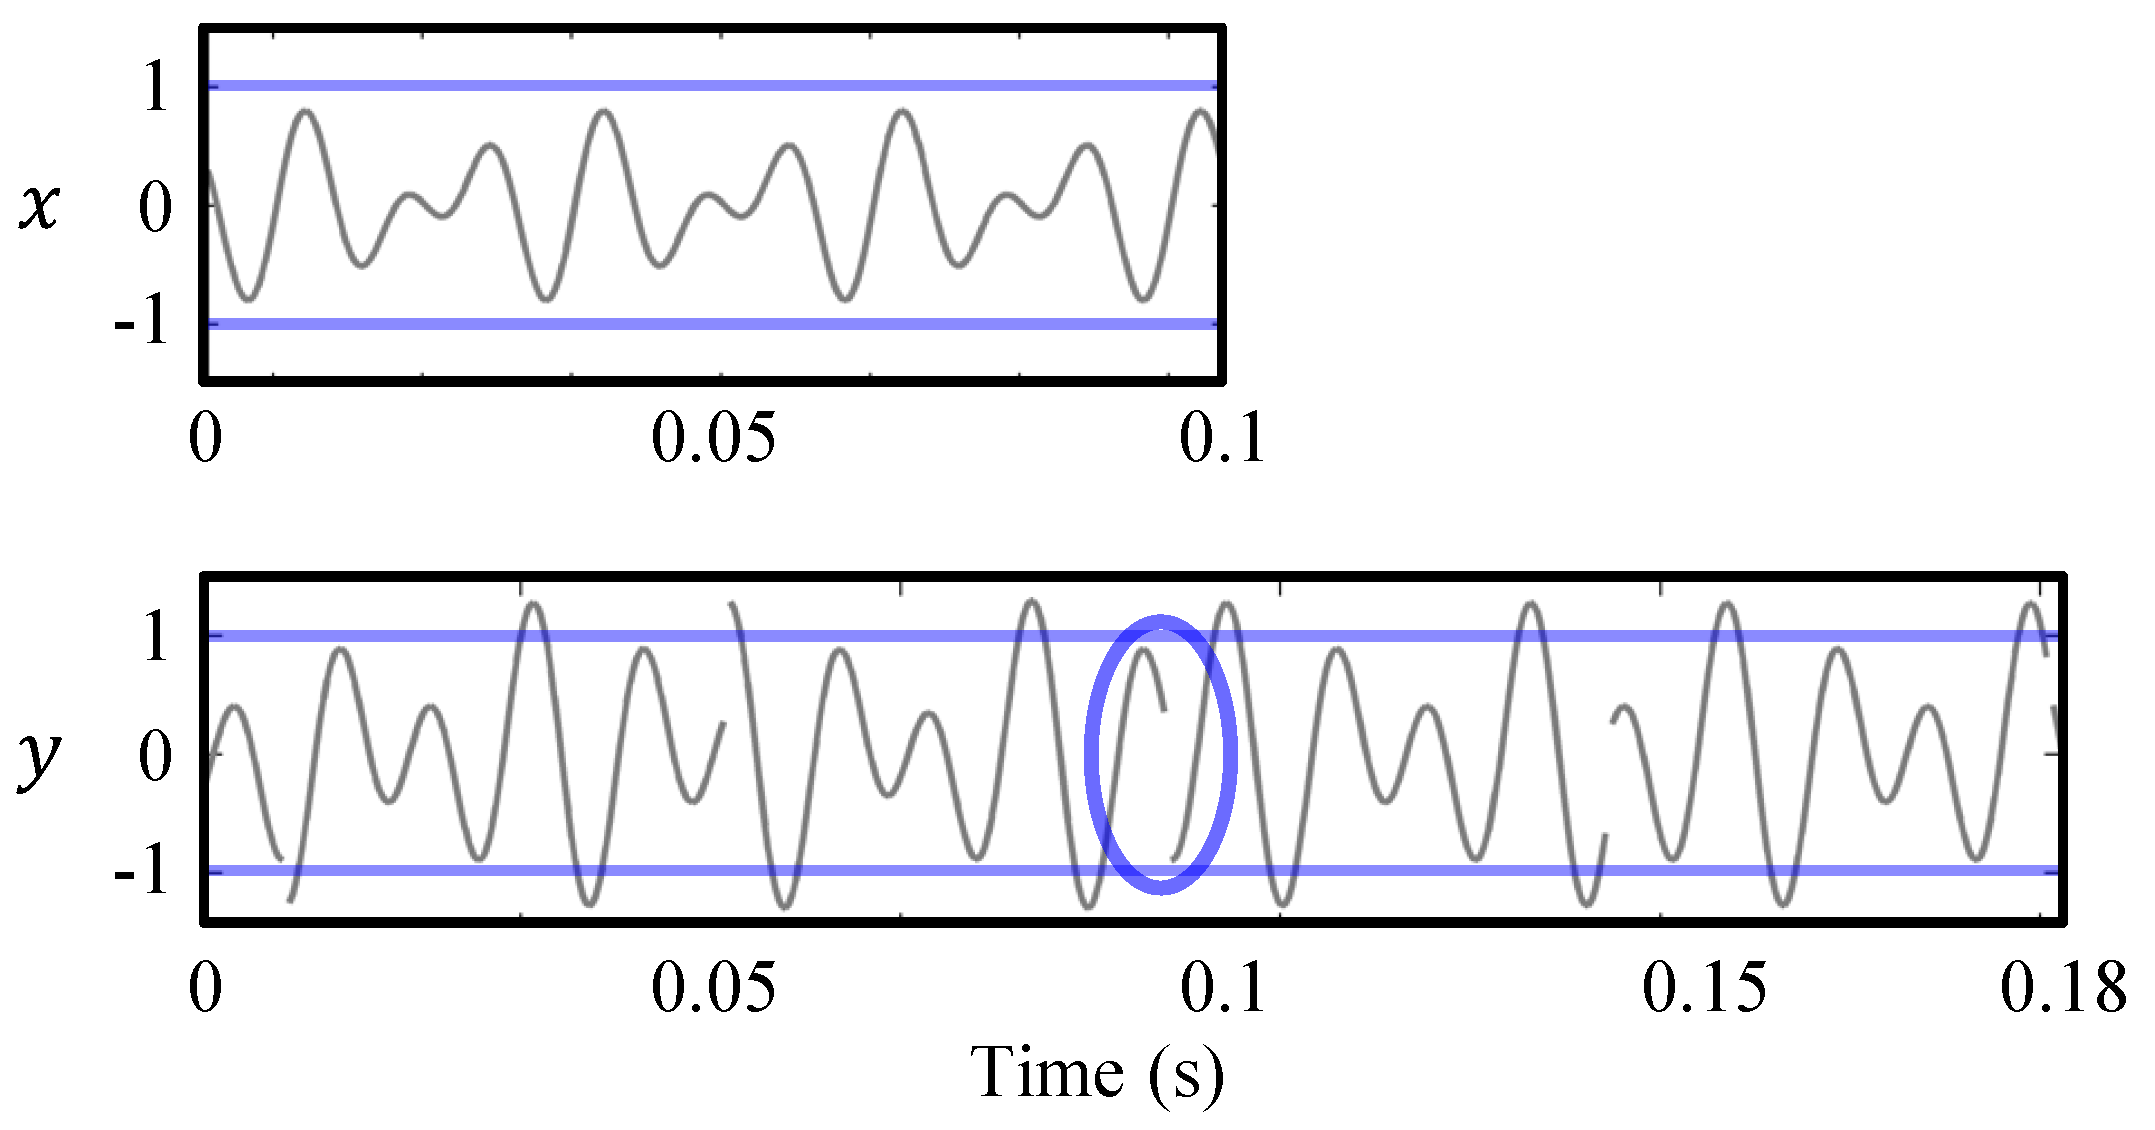
\includegraphics[width=9cm]{res/artifact.png}}
    \caption{\label{fig:artifact}Exemple d'artefact qui se produit quand le même grain d'analyse est
      utilisé pour reconstruire le signal avec le tempo modifié. \cite{TSMreview} }
  \end{figure}
  
L'algorithme \emph{OLA} se base sur cette méthode basique et rajoute des fénêtres pour avoir une
fluidité dans la transition d'un grain à un autre. Les grains $x_m$ sont donc appliqués à une fonction
de fênetrage $w$ \dots [a continuer demain]

\subsection{Méthode W/SOLA}

\subsection{Méthode vocodeur de phases}

\subsection{TD-PSOLA}

\begin{comment}
Parler de SOLA, PSOLA...
\end{comment}

\subsection{Traitement des fréquences}

\begin{comment}
  Parler du Vocodeur de phases, comment c'est utilisé etc...
\end{comment}
\subsection{Traitement du temps et des fréquences}
Des techniques SOLA peuvent déjà donner des 

\begin{comment}
  On parle des techniques comme PVSOLA -> SOLA en prenant en compte la phase etc
\end{comment}

\section{Méthodes}

Les 2 méthodes qui ont été développées sont la granulation et le vocodeur de phases.
Ces 2 méthodes ont été utilisées en utilisant la fonction le système de génération de
synthétiseurs ``defsynth'' d'Overtone.
\begin{comment}
  Parler d'Overtone, Supercollider...
  UGENs qu'on va utiliser: PVRecordBuf, PVPlayBuf..
\end{comment}

\subsection{Langages fonctionnels}
\begin{comment}
\end{comment}

\subsection{Overtone}
\begin{comment}
  Parler d'Overtone-supercollider, les methodes que ça nous donne etc
  [CITER ARTICLE SONICPI -> OVERTONE DE SAM AARON]
\end{comment}

\subsection{AWESOME OVERTONE TWEAK THINGS}
\subsection{SOLA approach / granulator}
[Expliquer ce que c'est un granulator]

Un granulator a été implementé sur Overtone en utilisant les UGENs suivants
de SuperCollider:


\subsection{Vocodeur de phases}


\section{Résultats}

\section{Remerciements}
  Je remercie mon prometeur, Bernard Fortz, de m'avoir fait découvrir
  les yeux au monde du live-coding et la programmation fonctionnelle.

  Je tiens aussi à remercier l'UrLab pour m'avoir accueilli au SmartMonday
  pour partager avec eux tout ce que j'ai appris lors de mes recherches
  pour ce mémoire.

  [Remerciements à Antoine]

\footnotesize

\bibliographystyle{apalike}
\bibliography{rapport}


\end{document}
